\experiment{Priority Queue}{14/11/2023}

\section{Aim}
To implement a program that represents a priority queue using an array.

\section{Algorithm}
 {\fontfamily{lmtt}\selectfont

  \subsection{Create Queue}
  \begin{enumerate}[label=\arabic*:,left=0pt]
    \item \textbf{Start}
    \item Create a structure \texttt{queue} with the following attributes:
          \begin{enumerate}[label=2.\arabic*:,left=0pt]
            \item Integer \texttt{size} to store the size of the queue.
            \item Integer \texttt{length} to store the current length of the queue.
            \item Integer array \texttt{arr[100]} to store the elements of the queue.
          \end{enumerate}
    \item Create a function \texttt{createQueue()}:
          \begin{enumerate}[label=3.\arabic*:,left=0pt]
            \item Allocate memory for a new \texttt{queue} structure using \texttt{malloc}.
            \item Set \texttt{length} to 0.
            \item Set \texttt{size} to 100.
            \item Return the created \texttt{queue} structure.
          \end{enumerate}
    \item \textbf{Stop}
  \end{enumerate}

  \subsection{Enqueue Function}
  Create a function \texttt{enqueue(q, value)}:
  \begin{enumerate}[label=\arabic*:,left=0pt]
    \item \textbf{Start}
    \item If \texttt{length} is equal to \texttt{size}, print "Queue overflow" and return.
    \item Declare integer \texttt{i} and initialize it to 0.
    \item Loop from \texttt{i} equal to 0 to \texttt{length - 1}:
          \begin{enumerate}[label=3.\arabic*:, start=1]
            \item If \texttt{q->arr[i] < value}, break from the loop.
          \end{enumerate}
    \item Loop from \texttt{k} equal to \texttt{length} to \texttt{i + 1}:
          \begin{enumerate}[label=4.\arabic*:, start=1]
            \item Set \texttt{q->arr[k]} to \texttt{q->arr[k - 1]}.
          \end{enumerate}
    \item Set \texttt{q->arr[i]} to \texttt{value}.
    \item Increment \texttt{length}.
    \item Call the \texttt{display} function.
    \item \textbf{Stop}
  \end{enumerate}

  \subsection{Dequeue Function}
  Create a function \texttt{dequeue(q)}:
  \begin{enumerate}[label=\arabic*:,left=0pt]
    \item \textbf{Start}
    \item Print the element at the front of the queue: \texttt{q->arr[0]}.
    \item Decrement \texttt{length}.
    \item Loop from \texttt{i} equal to 0 to \texttt{length - 1}:
          \begin{enumerate}[label=3.\arabic*:, start=1]
            \item Set \texttt{q->arr[i]} to \texttt{q->arr[i + 1]}.
          \end{enumerate}
    \item Call the \texttt{display} function.
    \item \textbf{Stop}
  \end{enumerate}

  \subsection{Display Function}
  Create a function \texttt{display(q)}:
  \begin{enumerate}[label=\arabic*:,left=0pt]
    \item \textbf{Start}
    \item Loop from \texttt{i} equal to 0 to \texttt{length - 1}:
          \begin{enumerate}[label=2.\arabic*:, start=1]
            \item Print \texttt{q->arr[i]}.
          \end{enumerate}
    \item Print a newline.
    \item \textbf{Stop}
  \end{enumerate}

  \subsection{ Peak Function }
  Create a function \texttt{peak(q)}:
  \begin{enumerate}[label=\arabic*:,left=0pt]
    \item \textbf{Start}
    \item Print the element at the front of the queue: \texttt{q->arr[0]}.
    \item \textbf{Stop}
  \end{enumerate}

  \subsection{Main Function}
  In the \texttt{main} function:
  \begin{enumerate}[label=\arabic*:, start=1]
    \item \textbf{Start}
    \item Call the \texttt{createQueue} function to create a new queue \texttt{q}.
    \item Declare an integer variable \texttt{ch}.
    \item Print the menu:
          \begin{enumerate}[label=3.\arabic*:, start=1]
            \item Print "1) Enqueue".
            \item Print "2) Dequeue".
            \item Print "3) Peek".
            \item Print "4) Display".
            \item Print "5) Exit".
          \end{enumerate}
    \item Loop while \texttt{ch != 5}:
          \begin{enumerate}[label=5.\arabic*:, start=1]
            \item Print "Choice: ".
            \item Take user input for \texttt{ch}.
            \item If \texttt{ch == 1}, take user input for \texttt{x} and call \texttt{enqueue(q, x)}.
            \item If \texttt{ch == 2}, call \texttt{dequeue(q)}.
            \item If \texttt{ch == 3}, call \texttt{peak(q)}.
            \item If \texttt{ch == 4}, call \texttt{display(q)}.
            \item If \texttt{ch != 5}, print "Invalid option!".
          \end{enumerate}
    \item \textbf{Stop}
  \end{enumerate}
 }

\section{C Program}
\begin{lstlisting}[label={list:c_program:priority_queue}]
#include <stdlib.h>
#include <stdio.h>

typedef struct queue
{
  int size;
  int length;
  int arr[100];
} queue;

queue *createQueue();
void enqueue(queue *q, int value);
void dequeue(queue *q);
void peak(queue *q);
void display(queue *q);

int main()
{
  queue *q = createQueue();
  int ch;
  printf("1)Enqueue\n2)Dequeue\n3)Peek\n4)Display\n5)Exit\n");
  do
  {
    printf("Choice: ");
    scanf("%d", &ch);
    if (ch == 1)
    {
      int x;
      printf("\nEnter the data: ");
      scanf("%d", &x);
      enqueue(q, x);
    }
    else if (ch == 2)
    {
      dequeue(q);
    }
    else if (ch == 3)
    {
      peak(q);
    }
    else if (ch == 4)
    {
      display(q);
    }
    else if (ch != 5)
    {
      printf("\nInvalid option!\n");
    }
  } while (ch != 5);
}

queue *createQueue()
{
  queue *q = (queue *)malloc(sizeof(queue));
  q->length = 0;
  q->size = 100;
  return q;
}

void enqueue(queue *q, int value)
{
  if (q->length == q->size)
  {
    printf("\nQueue overflow\n");
  }
  int i = 0;
  for (i = 0; i < q->length; i++)
  {
    if (q->arr[i] < value)
    {
      break;
    }
  }
  for (int k = q->length; k > i; k--)
  {
    q->arr[k] = q->arr[k - 1];
  }
  q->arr[i] = value;
  q->length++;
  display(q);
}

void dequeue(queue *q)
{
  printf("\n%d dequeued\n", q->arr[0]);
  q->length--;
  for (int i = 0; i < q->length; i++)
  {
    q->arr[i] = q->arr[i + 1];
  }
  display(q);
}

void display(queue *q)
{
  for (int i = 0; i < q->length; i++)
  {
    printf("%d ", q->arr[i]);
  }
  printf("\n");
}

void peak(queue *q)
{
  printf("\n%d\n", q->arr[0]);
}
\end{lstlisting}

\section{Output}
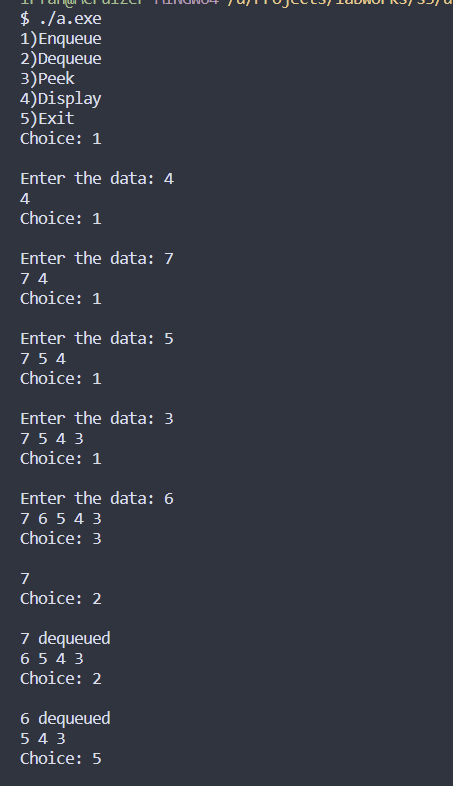
\includegraphics[]{Cycle_1/Outputs/PriorityQueue.png}

\section{Result}
The priority queue was implemented successfully using an array, program is executed and output is verified.